%-------------------------------------------------------
\begin{frame}{Introduction}{A general view about the Data Mining process}
%-------------------------------------------------------
	\noindent\begin{centering}
		\vspace{-2mm}\hspace{-5mm}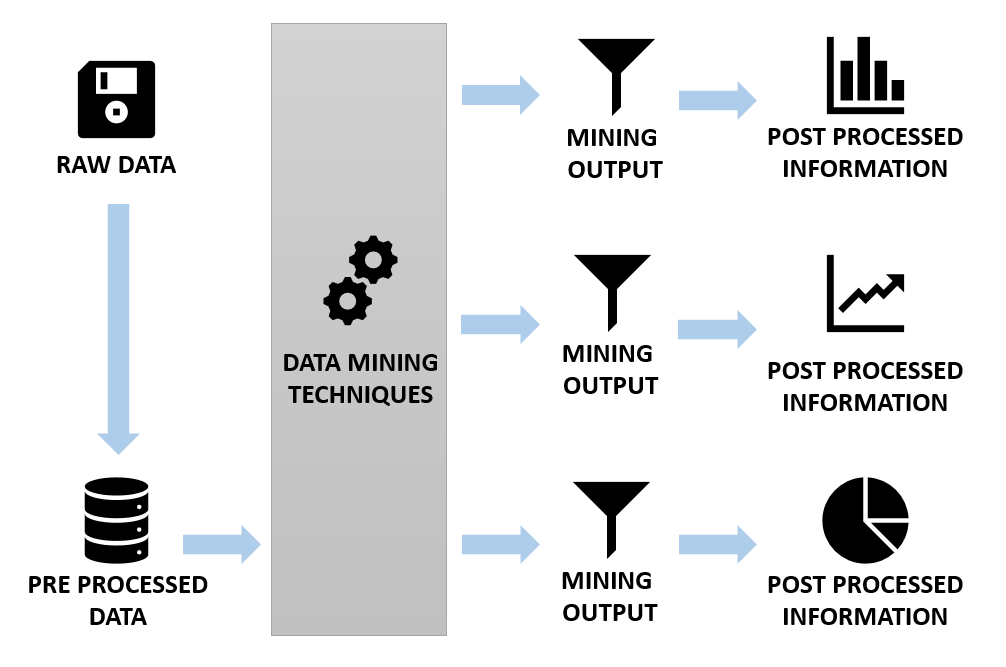
\includegraphics[scale=0.33]{img1_noback.png}
	\end{centering}
\end{frame}

%-------------------------------------------------------
\begin{frame}{Introduction}{The choice of appropriate technologies}
%-------------------------------------------------------

	\centering\textit{Which technology should be employed?} \vspace{0,3cm}

	\begin{block}{}
	    \begin{itemize}
		    \item<1-> \alert{Data Processing} --- \textbf{MongoDB}: advanced \emph{dbms}, operating in the \emph{noSQL} paradigm. \\ \hspace{0.8cm}\textcolor{cyan}{\emph{new!}}
		    \item<2-> \alert{Data Mining Algorithms} --- \textbf{Weka}: software which provide a \emph{framework} for running data mining algorithms.
			\item<3-> \alert{Visualization Techniques} \\
			--- \textbf{R language}: programming language with an extensive data visualization library; \\
			--- \textbf{Spreadsheets}: tabular data managing software, like Microsoft Excel and OpenOffice Calc.
	    \end{itemize}
    \end{block}

\end{frame}
